\documentclass{article}
\usepackage{latexsym}
\usepackage{amsfonts}
\usepackage[pdftex]{graphicx}
\graphicspath{{pictures/}}
\DeclareGraphicsExtensions{.pdf,.png,.jpg}
\usepackage{cmap}
\usepackage[T2A]{fontenc}
\usepackage[utf8]{inputenc}
\usepackage[english, russian]{babel}
\usepackage{pdfpages}


\begin{document}

\begin{flushright}

\Large Горелкина \\ РК6-32Б \\ Вариант №4

\end{flushright}

\vspace{\baselineskip}\vspace{\baselineskip}\vspace{\baselineskip}\vspace{\baselineskip}\vspace{\baselineskip}\vspace{\baselineskip}\vspace{\baselineskip}\vspace{\baselineskip}\vspace{\baselineskip}

\begin{center}

\section*{Домашнее задание №2 по курсу теории вероятностей и математической статистики. \\ Часть №1. Дискретные случайные величины.}

\vspace{\baselineskip}
\textbf{\large Исходные данные}
\vspace{\baselineskip}

\begin{tabular}[c]{p{0.5cm}|p{0.5cm}|p{0.5cm}|p{0.5cm}|p{0.5cm}|p{0.5cm}|p{0.5cm}|p{0.5cm}|p{0.5cm}}
\textbf{\begin{math}R_1\end{math}} & \textbf{\begin{math}G_1\end{math}} & \textbf{\begin{math}B_1\end{math}} & \textbf{\begin{math}R_2\end{math}} & \textbf{\begin{math}G_2\end{math}} & \textbf{\begin{math}B_2\end{math}} & \textbf{\begin{math}R_3\end{math}} & \textbf{\begin{math}G_3\end{math}} & \textbf{\begin{math}B_3\end{math}} 
\\[1mm] \hline
11 & 6 & 8 & 10 & 5 & 10 & 8 & 5 & 6  
\end{tabular}

\end{center}
\vspace{\baselineskip}\vspace{\baselineskip}\vspace{\baselineskip}\vspace{\baselineskip}\vspace{\baselineskip}\vspace{\baselineskip}\vspace{\baselineskip}\vspace{\baselineskip}\vspace{\baselineskip}\vspace{\baselineskip}\vspace{\baselineskip}\vspace{\baselineskip}\vspace{\baselineskip}\vspace{\baselineskip}\vspace{\baselineskip}\vspace{\baselineskip}\vspace{\baselineskip}\vspace{\baselineskip}\vspace{\baselineskip}\vspace{\baselineskip}
\textbf {\largeЗадача 1.} 
\large Рассматривается извлечение шаров с возвращением из первой корзины. Выполняется серия из \begin{math}n\end{math} экспериментов, подсчитывается число \begin{math}k\end{math} извлечений красных шаров.
\vspace{\baselineskip}
\\
\large 1. Построить графики вероятности \begin{math}P(k)\end{math}. Графики строятся для числа опытов \begin{math}n = 6,\ 9,\ 12\end{math} c расчётом вероятностей по формуле Бернулли.
\vspace{\baselineskip}
\\
\large 2. Для \begin{math}n = 6\end{math} также строится график функции распределения \begin{math}F(x)\end{math}.
\vspace{\baselineskip}
\\
\large 3. Для \begin{math}n = 25,\ 50,\ 100,\ 200,\ 400,\ 1000\end{math} строится огибающая графика \begin{math}P(k)\end{math}, при этом для каждого графика рассчитываются не менее \begin{math}7\end{math} точек с использованием локальной теоремы Муавра-Лапласа.
\vspace{\baselineskip}
\\
\large 4. Построить график вероятности того, что абсолютное число извлечений красных шаров отклонится от математического ожидания не более, чем на \begin{math}R_1\end{math}. При построении графика использовать \begin{math}n = 25,\ 50,\ 100\end{math}.
\vspace{\baselineskip}
\\
\large 5. Построить график вероятности того, что относительное число извлечений красных шаров отклонится от математического ожидания не более, чем на \begin{math}\displaystyle\frac{R_1}{R_1 + G_1 + B_1}\end{math}. При построении графика использовать \begin{math}n = 100, \ 200,\  400\end{math}.
\vspace{\baselineskip}
\\
\large 6. Рассчитать допустимый интервал числа успешных испытаний k (симметричный относительно математического ожидания), обеспечивающий попадание в него с вероятностью \begin{math}P = \displaystyle\frac{R_1}{R_1 + G_1 + B_1}\end{math} при \begin{math}n = 1000\end{math}.
\vspace{\baselineskip}
\\
\large 7. Построить график зависимости минимально необходимого числа испытаний n, для того, чтобы обеспечить вероятность появления не менее, чем \begin{math}N_1 = R_1 + G_1 + B_1\end{math} красных шаров с вероятностями \begin{math}P = 0.7,\ 0.8,\ 0.9,\ 0.95\end{math}.
\vspace{\baselineskip}
\\
\vspace{\baselineskip}
\\
\textbf{Решение:}
\vspace{\baselineskip}
\\
I. Для построения графиков запишем в общем виде функцию \begin{math}P(k)\end{math} по формуле Бернулли для произвольного числа испытаний \begin{math}n\end{math}, а затем построим необходимые частные случаи.
\begin{center}
\begin{math}P(k) = C^k_n \cdot \left(\displaystyle\frac{R_1}{R_1 + G_1 + B_1}\right)^k \cdot \left(1 - \displaystyle\frac{R_1}{R_1 + G_1 + B_1}\right)^{n-k} =  \end{math}
\vspace{\baselineskip}
\\
\begin{math} = C^k_n \cdot \left(\displaystyle\frac{11}{25}\right)^k \cdot \left(1 - \displaystyle\frac{11}{25}\right)^{n-k} = C^k_n \cdot \left(\displaystyle\frac{11}{25}\right)^k \cdot \left(\displaystyle\frac{14}{25}\right)^{n-k} \end{math}
\end{center}
\vspace{\baselineskip}
Мы получили выражение для \begin{math}P(k)\end{math}. Для построения графиков будет использован математический пакет \begin{math}MATLAB\end{math}. Скрипт и графики с таблицами значений функций вероятностей находятся в приложении 1.1.
\vspace{\baselineskip}
\\
II. По определению функции распределения \begin{math}F(x) = \sum P_i\end{math}. Значения \begin{math}P_i\end{math} уже найдены. Для построения графика будет использован математический пакет \begin{math}MATLAB\end{math}. Скрипт и график с таблицей значений функции распределения находятся в приложении 1.1.
\vspace{\baselineskip}
\\
III. Локальная теорема Муавра-Лапласа:
\vspace{\baselineskip}
\\
\begin{math}
P(X=k)  \approx \displaystyle\frac{1}{\sqrt{npq}} \varphi \left(  \displaystyle\frac{k-np}{\sqrt{npq}} \right)
\end{math}. Для построения огибающих воспользуемся центральной предельной теоремой, из которой следует: \begin{math}
Bin(n, p) \approx N(np, npq).  \ N = \displaystyle\frac{1}{\sigma \sqrt{2 \pi}}\cdot e^\frac{-(x - \mu)^2}{2\sigma^2}
\end{math} - распределение Гаусса.
\vspace{\baselineskip}
\\Дальнейшие вычисления и графики находятся в приложении 1.2. Для их построения был использован язык программирования \begin{math}
 Python \ 3.8.1
\end{math}. 
\vspace{\baselineskip}
\\
IV. Вероятность того, что случайная величина будет попадать в некоторый интервал \begin{math}
\left( k_1, k_2 \right)
\end{math} при достаточно большом количестве испытаний \begin{math} n \end{math} находится с помощью интегральной теоремы Муавра-Лапласа и равна
\begin{math}
{{P}_{n}}\left( {{k}_{1}},{{k}_{2}} \right)\approx \Phi \left( \displaystyle\frac{{{k}_{2}}-np}{\sqrt{npq}} \right)-\Phi \left( \displaystyle\frac{{{k}_{1}}-np}{\sqrt{npq}} \right)\
\end{math}. В нашем случае требуется построить график \begin{math}
{{P}_{n}}\left( {|k - M(k)| \leq R_1} \right)
\end{math}. Данная функция будет зависеть от \begin{math}
n
\end{math},  а график построим по трём точкам. Известно, что вероятность схемы Бернулли подчиняется биномиальному закону распределения. Поэтому \begin{math} M(k) = n \cdot p \end{math} и   \begin{math}
{{P}_{n}}\left( {|k - n\cdot p | \leq R_1} \right)
 = 2\cdot\Phi \left( \displaystyle\frac{R_1}{\sqrt{npq}}\right)\end{math}.Расчёты необходимых вероятностей реализованы с помощью языка программирования \begin{math}
 Python \ 3.8.1
\end{math} и таблицы со значениями функции Лапласа и находятся в приложении 1.2. 
\vspace{\baselineskip}
\\
V. Аналогично пункту IV воспользуемся интегральной теоремой Муавра-Лапласа. Только в данном случае, так как мы берем случайную величину \begin{math}
\displaystyle\frac{k}{n}
\end{math}, то и матожидание возьмём \begin{math}
M\left(\displaystyle\frac{k}{n}\right) = \displaystyle\frac{M(k)}{n} = \displaystyle\frac{n\cdot p}{n} = p
\end{math}. Получаем, что
\vspace{\baselineskip}
\\
\begin{math}{{P}_{n}}\left( {\left|\displaystyle\frac{k}{n} - p \right| \leq \displaystyle\frac{R_1}{N_1}} \right)
 = 2\cdot\Phi \left( \displaystyle\frac{n \cdot R_1}{N_1\cdot\sqrt{npq}}\right)\end{math}. Расчёты необходимых вероятностей реализованы с помощью языка программирования \begin{math}
 Python \ 3.8.1
\end{math} и таблицы со значениями функции Лапласа и находятся в приложении 1.2. 
\vspace{\baselineskip}
\\
VI. Пусть у нас имеется некоторый интервал \begin{math}
(M(k) - \alpha, M(k) + \alpha)
\end{math}, симметричный относительно матожидания. Тогда вероятность попадания величины \begin{math}
k
\end{math} в этот интервал равна (по интегральной теореме Муавра-Лапласа):
\begin{math}
P_n((M(k) - \alpha \leq k \leq M(k) + \alpha) = P_n(|k - M(k)| \leq \alpha) = P_n(|k - n\cdot p| \leq \alpha) = P_n\left(\left| \displaystyle\frac{k}{n}- p\right| \leq \displaystyle\frac{\alpha}{n}\right) = 2\cdot\Phi\left(\displaystyle\frac{\alpha}{\sqrt{p \cdot q\cdot n}}\right).
\end{math} По условию \begin{math}
P_n = \displaystyle\frac{11}{25} = 2\cdot\Phi\left(\displaystyle\frac{\alpha}{\sqrt{\displaystyle\frac{11}{25} \cdot \displaystyle\frac{14}{25}\cdot 1000}}\right) 
\end{math}. Тогда \begin{math}\Phi\left(\displaystyle\frac{25 \cdot\alpha}{10 \cdot \sqrt{11 \cdot 14 \cdot 10}}\right) = \displaystyle\frac{11}{50}  = 0.22\end{math}. По таблице значений функции Лапласа находим, что аргумент равен 0.58. То есть \begin{math}
 \displaystyle\frac{\sqrt{385} \cdot\alpha}{308}= 0.58 \Leftrightarrow \alpha = \displaystyle\frac{58 \cdot\sqrt{385}}{125} \approx 9.104
\end{math}. Таким образом, получаем интервал \begin{math}
(M(k) - 9.104, M(k) + 9.104)
\end{math}, \begin{math}
M(k) = n \cdot p = \displaystyle\frac{1000 \cdot 11}{25} = 440.
\end{math} Искомый интервал равен \begin{math}
(430.896, \ 449.104)
\end{math}.
\vspace{\baselineskip}
\\
VII. Снова воспользуемся интегральной теоремой Муавра-Лапласа. Будем находить следующую вероятность \begin{math}
P_n(N_1 \leq k),
\end{math} которая должна принимать указанные в условии значения. Так как испытаний должно быть максимум \begin{math}
n
\end{math}, то можем переписать вероятность следующим образом \begin{math}
P_n(N_1 \leq k \leq n) = \Phi(x_2) - \Phi(x_1), \ x_2 = \\ = \displaystyle\frac{n - n\cdot p}{\sqrt{n \cdot p \cdot q}}, \ x_1 = \displaystyle\frac{25 - n\cdot p}{\sqrt{n \cdot p \cdot q}}.
\end{math} Понятно, что \begin{math}
 \ x_2 \geq \displaystyle\frac{25 - 25\cdot \displaystyle\frac{11}{25}}{\sqrt{25 \cdot\displaystyle\frac{11}{25} \cdot \displaystyle\frac{14}{25}}} \approx \\ \approx 5.64
\end{math}. То есть фактически \begin{math}
\Phi(x_2) \approx 0.5 \end{math}. Это дает нам возможность вычислить значения \begin{math}
\Phi(x_1) \end{math} для четырех заданных значений \begin{math}
P_n. \end{math}
\vspace{\baselineskip}
\\
Первый случай \begin{math}
P_n = 0.7:  \ \Phi(x_1) = 0.5 -  0.7 = - 0.2, \ x_1 = -0.52 = \displaystyle\frac{625 - 11\cdot n}{\sqrt{154 \cdot n}}, \ n = 62 \end{math}.
\vspace{\baselineskip}
\\
Второй случай \begin{math}
P_n = 0.8:  \ \Phi(x_1) = 0.5 - 0.8 = -0.3, \ x_1 = -0.84 = \displaystyle\frac{625 - 11\cdot n}{\sqrt{154 \cdot n}}, \ n = 65 \end{math}.
\vspace{\baselineskip}
\\
Третий случай \begin{math}
P_n = 0.9:  \ \Phi(x_1) = 0.5 - 0.9 = -0.4, \ x_1 = -1.28 = \displaystyle\frac{625 - 11\cdot n}{\sqrt{154 \cdot n}}, \ n = 69 \end{math}.
\vspace{\baselineskip}
\\
Четвёртый случай \begin{math}
P_n = 0.95:  \ \Phi(x_1) = 0.5 - 0.95 = -0.45, \ x_1 = \\ = -1.64 = \displaystyle\frac{625 - 11\cdot n}{\sqrt{154 \cdot n}}, \ n = 73 \end{math}.
\vspace{\baselineskip}
\\
Дальнейшее построение графика выполнено с помощью языка программирования \begin{math}
 Python \ 3.8.1
\end{math} скрипт и график находятся в приложении 1.2.
\vspace{\baselineskip}\vspace{\baselineskip}\vspace{\baselineskip}\vspace{\baselineskip}\vspace{\baselineskip}\vspace{\baselineskip}\vspace{\baselineskip}\vspace{\baselineskip}
\\
\textbf {\largeЗадача 2.} 
\large Рассматривается извлечение шаров без возвращения из второй корзины  Выполняется серия из \begin{math}n=G_2+B_2\end{math} экспериментов, подсчитывается число \begin{math}k\end{math} извлечений красных шаров.
\vspace{\baselineskip}
\\
\large 1. Построить график вероятности \begin{math}P(k)\end{math}.
\vspace{\baselineskip}
\\
\large 2. Построить график функции распределения \begin{math}F(x)\end{math}.
\vspace{\baselineskip}
\\
\large 3. Рассчитать математическое ожидание числа извлечённых красных шаров \begin{math}k\end{math}.
\vspace{\baselineskip}
\\
\large 4. Рассчитать дисперсию числа извлечённых красных шаров \begin{math}k\end{math}.
\vspace{\baselineskip}
\\
\textbf{Решение:}
\vspace{\baselineskip}
\\
Для данного варианта \begin{math}
n = 15
\end{math}, красных шаров \begin{math}
R_2 = 10
\end{math} во второй корзине, а всего  шаров во второй корзине \begin{math}
N_2 = 25.
\end{math}
Для построения графиков запишем в общем виде формулу для \begin{math}P(k)\end{math}.
\vspace{\baselineskip}
\\
\begin{center}
\begin{math}
P(k) = \displaystyle\frac{\displaystyle{k \choose R_2} \cdot {n-k \choose G_2 + B_2}}{\displaystyle{n \choose R_2 + G_2 + B_2}} = \displaystyle\frac{R_2! \cdot n! \cdot R_2! \cdot n!}{N_2! \cdot k! \cdot (n-k)! \cdot (R_2 - k)! \cdot k!} = 
\end{math}
\vspace{\baselineskip}
\\
\begin{math}
= \displaystyle\frac{10! \cdot 10! \cdot 15! \cdot 15! }{25! \cdot k! \cdot k! \cdot (10 - k)! \cdot (15 - k)!} = 
\end{math}
\vspace{\baselineskip}
\\
\begin{math} =\displaystyle\frac{1}{3268760} \cdot \displaystyle\frac{15!}{k! \cdot (15 - k)!} \cdot \displaystyle\frac{10!}{k! \cdot (10-k)!}
\end{math}
\vspace{\baselineskip}
\\
\end{center}
Последние 2 множителя в аналитическом выражении легко можно задать неким рекуррентным соотношением \begin{math}
 F_{k} = F_{k-1} \cdot \displaystyle\frac{10- k}{k+1} 
\end{math} и \begin{math}
 F_{k} = F_{k-1} \cdot \displaystyle\frac{15- k}{k+1} 
\end{math} для \begin{math}
 k \geq 1
\end{math}, для \begin{math}
 k = 0 
\end{math} будем считать, что 
\begin{math}
 F_{k} = 1.
 \end{math}
\vspace{\baselineskip}
\\
Матожидание и дисперсию случайной величины будем считать по формулам для гипергеометрического распределения:
\vspace{\baselineskip}
\\
\begin{math}
M(k) = \displaystyle\frac{n\cdot R_2}{N_2}, \ \ \  D(k) = \displaystyle\frac{n\cdot \displaystyle\frac{R_2}{N_2} \cdot \left( 1 - \displaystyle\frac{R_2}{N_2} \right) \cdot (N_2 - n)}{N_2 - 1}.
\end{math}
\vspace{\baselineskip}
\\
Дальнейшие вычисления были осуществлены с помощью языка программирования \begin{math}
 Python \ 3.8.1
\end{math}. Скрипт с графиками функций и вычислениями находится в приложении 2.
\vspace{\baselineskip}\vspace{\baselineskip}\vspace{\baselineskip}\vspace{\baselineskip}\vspace{\baselineskip}\vspace{\baselineskip}\vspace{\baselineskip}\vspace{\baselineskip}\vspace{\baselineskip}\vspace{\baselineskip}\vspace{\baselineskip}\vspace{\baselineskip}\vspace{\baselineskip}\vspace{\baselineskip}\vspace{\baselineskip}\vspace{\baselineskip}\vspace{\baselineskip}\vspace{\baselineskip}\vspace{\baselineskip}\vspace{\baselineskip}\vspace{\baselineskip}\vspace{\baselineskip}\vspace{\baselineskip}\vspace{\baselineskip}\vspace{\baselineskip}\vspace{\baselineskip}\vspace{\baselineskip}\vspace{\baselineskip}\vspace{\baselineskip}\vspace{\baselineskip}\vspace{\baselineskip}\vspace{\baselineskip}\vspace{\baselineskip}\vspace{\baselineskip}
\\
\textbf {\largeЗадача 3.} 
\large Рассматривается извлечение шаров без возвращения из третьей корзины. Выполняется серия из \begin{math}k\end{math} экспериментов, которая прекращается, когда извлечены все \begin{math}R_3\end{math} красных шаров.
\vspace{\baselineskip}
\\
\large 1. Рассчитать значения \begin{math}P(k)\end{math}.
\vspace{\baselineskip}
\\
\large 2. Рассчитать математическое ожидание числа извлечений \begin{math}k\end{math}.
\vspace{\baselineskip}
\\
\large 3. Рассчитать дисперсию числа извлечений \begin{math}k\end{math}
\vspace{\baselineskip}
\\
\textbf{Решение:}
\vspace{\baselineskip}
\\
Заметим, что \begin{math}k\end{math} не может быть меньше \begin{math}R_3 = 8\end{math}. Также очевидно, \begin{math}k\end{math} не может быть больше \begin{math}N_3 = R_3 + G_3 + B_3 = 19 \end{math}. Поэтому для целого \begin{math}k \in \left(-\infty, 7] \ \cup \ [20, +\infty \right) \  P(k) = 0\end{math}.
Чтобы найти необходимые значения вероятностей, будем рассуждать так: последний извлеченный из корзины шар должен быть красным и при этом последним из красных. Поэтому, если учесть, что было проведено всего \begin{math}k\end{math} экспериментов, то до извлечения последнего шара было проведено, соответственно, \begin{math}k-1\end{math} экспериментов. Отсюда найдём вероятность того, что последний извлеченный шар оказался красным и последним из красных пи \begin{math}k\end{math} экспериментах: \begin{math} \displaystyle\frac{1}{N_3 - (k - 1)}\end{math}. Тогда среди извлеченных до этого шаров должно быть \begin{math}R_3 - 1\end{math} красных шаров. Понятно, что вероятность достать 7 красных шаров из 19 без возвращения будет равна \begin{math}\displaystyle\frac{8 \cdot 7 \cdot 6 \cdot 5 \cdot 4 \cdot 3 \cdot 2}{19 \cdot 18 \cdot 17 \cdot 16 \cdot 15 \cdot 14 \cdot 13} = \displaystyle\frac{8! \cdot 12!}{19!} = \left(N_3 - R_3 + 1 \right) \cdot \displaystyle{R_3 \choose N_3}^{-1} \end{math}. При этом было извлечено ещё некоторое количество шаров синего и зелёного цветов, вероятность этого события будет равна \begin{math}\displaystyle\frac{11 \cdot 10 \cdot 9 ...}{12 \cdot 11 \cdot 10 ...} = \displaystyle\frac{N_3 - (k - 1)}{N_3 - (R_3 - 1)}\end{math}. Важно ещё учесть, что зелёные и синие шары (а мы их в общем-то не различем) могли быть извлечены в различных комбинациях с красными шарами. Всего расположить \begin{math}k-  1 - R_3+1 \end{math} шаров на  \begin{math}k- 1 \end{math} позициях существует \begin{math}\displaystyle{k - R_3 \choose k - 1} \end{math} способов. Составим аналитическое выражене для \begin{math}P(k)\end{math} и упростим его:
\vspace{\baselineskip}
\\
\begin{center}
\begin{math}
P(k) = \displaystyle{k - R_3 \choose k - 1} \cdot
\displaystyle\frac{N_3 - k + 1}{N_3 - R_3 + 1} \cdot \displaystyle{R_3 \choose N_3}^{-1} \cdot \displaystyle\frac{N_3 - R_3 + 1}{N_3 - k + 1} = 
\end{math}
\vspace{\baselineskip}
\\
\begin{math}
 = \displaystyle\frac{(k-1)! \cdot R_3! \cdot (N_3 - R_3)!}{(k - R_3)! \cdot (R_3 - 1)! \cdot N_3!} = \displaystyle\frac{8! \cdot 11! \cdot (k-1)!}{ 7! \cdot 19!\cdot (k - R_3)!}
 = \end{math}

 \vspace{\baselineskip}
\\
 \begin{math} =\displaystyle\frac{1}{75582} \cdot \left( \displaystyle\frac{(k-1)!}{7! \cdot (k - 8)!} \right)\end{math}
  \end{center}
\vspace{\baselineskip}
\\
Рассмотрим альтернативное решение данной задачи. Будем решать следующую задачу: пусть все наши \begin{math} N_3 \end{math} шаров расположены в виде некоторой цепочки из красных и некрасных шаров (зелёных и синих, но мы их не различаем). \begin{math}
k
\end{math}-ая позиция в цепочке означает \begin{math}
k
\end{math}-ое извлечение. Чтобы посчитать количество всех возможных таких цепочек, найдем сочетание \begin{math}
\displaystyle{R_3 \choose N_3}
\end{math}. По условию нам требуется, чтобы на \begin{math}
k
\end{math}-ом извлечении мы достали последний красный шар. Поэтому разобьём нашу цепочку на две части. Первая часть будет состоять из \begin{math}
k - 1
\end{math} шара, а вторая часть будет состоять из \begin{math}
n - (k -1) = n - k + 1
\end{math} шара. Среди \begin{math}
k - 1
\end{math} шара у нас должно быть \begin{math}
R_3 - 1
\end{math} красных шара. Первая часть цепочки является аналогом событий, происходящих до \begin{math}k
\end{math}-го извлечения. Количество возможных первых частей цепочки, подходящих под условие, равно \begin{math}
\displaystyle{R_3 - 1 \choose k - 1}
\end{math}. Вторая часть цепочки содержит один красный шар. Но мы знаем, что он располагается только в одной позиции, то есть \begin{math}
k
\end{math}-ой. Поэтому общая вероятность будет равна
\begin{center}
    \begin{math}
    P(k) = \displaystyle\frac{\displaystyle{R_3 - 1 \choose k - 1}}{\displaystyle{R_3 \choose N_3}} = \displaystyle\frac{(k-1)! \cdot R_3! \cdot (N_3 - R_3)!}{(k - R_3)! \cdot (R_3 - 1)! \cdot N_3!} = \displaystyle\frac{8! \cdot 11! \cdot (k-1)!}{ 7! \cdot 19!\cdot (k - R_3)!} = \displaystyle\frac{1}{75582} \cdot \left( \displaystyle\frac{(k-1)!}{7! \cdot (k - 8)!} \right)
    \end{math}.
\end{center}
\vspace{\baselineskip}
\\
Второй множитель в получившемся выражении можно упростить, если рассматривать его значения для различных \begin{math}
 k = 8, \ 9, \ 10 \ ...
\end{math}
\\
Для \begin{math}
 k = 8
\end{math} имеем \begin{math}
\displaystyle\frac{7!}{0! \cdot 7!} = \displaystyle\frac{7}{7} = 1
\end{math}. 
\\
Для \begin{math}
 k = 9
\end{math} имеем \begin{math}
\displaystyle\frac{8!}{1! \cdot 7!} = \displaystyle\frac{8}{1} = 8.
\end{math}
\\
Для \begin{math}
 k = 10
\end{math} имеем \begin{math}
\displaystyle\frac{9!}{7! \cdot 2!} = \displaystyle\frac{9 \cdot 8 }{2 \cdot 1} = 36.
\end{math}
\vspace{\baselineskip}
\\
Заметим закономерность: данный множитель можно задать неким рекуррентным соотношением \begin{math}
 F_{k} = F_{k-1} \cdot \displaystyle\frac{k-1}{k-8} 
\end{math} для \begin{math}
 k \geq 9
\end{math}, для \begin{math}
 k = 8 
\end{math} будем считать, что 
\begin{math}
 F_{k} = 1.
\end{math}
\vspace{\baselineskip}
\\
Матожидание и дисперсию случайной величины будем считать по формулам:
\vspace{\baselineskip}
\\
\begin{math}
M(k) = \sum k \cdot P(k), \ \ \  D(k) = M(k^2) - M^2(k).
\end{math}
\vspace{\baselineskip}
\\
Дальнейшие вычисления были осуществлены с помощью языка программирования \begin{math}
 Python \ 3.8.1
\end{math}. Скрипт и результаты находятся в приложении 3.
\vspace{\baselineskip}
\includepdf[pages=-]{prob_1_12.pdf}
\includepdf[pages=-]{prob_12.pdf}
\includepdf[pages=-]{prob_2.pdf}
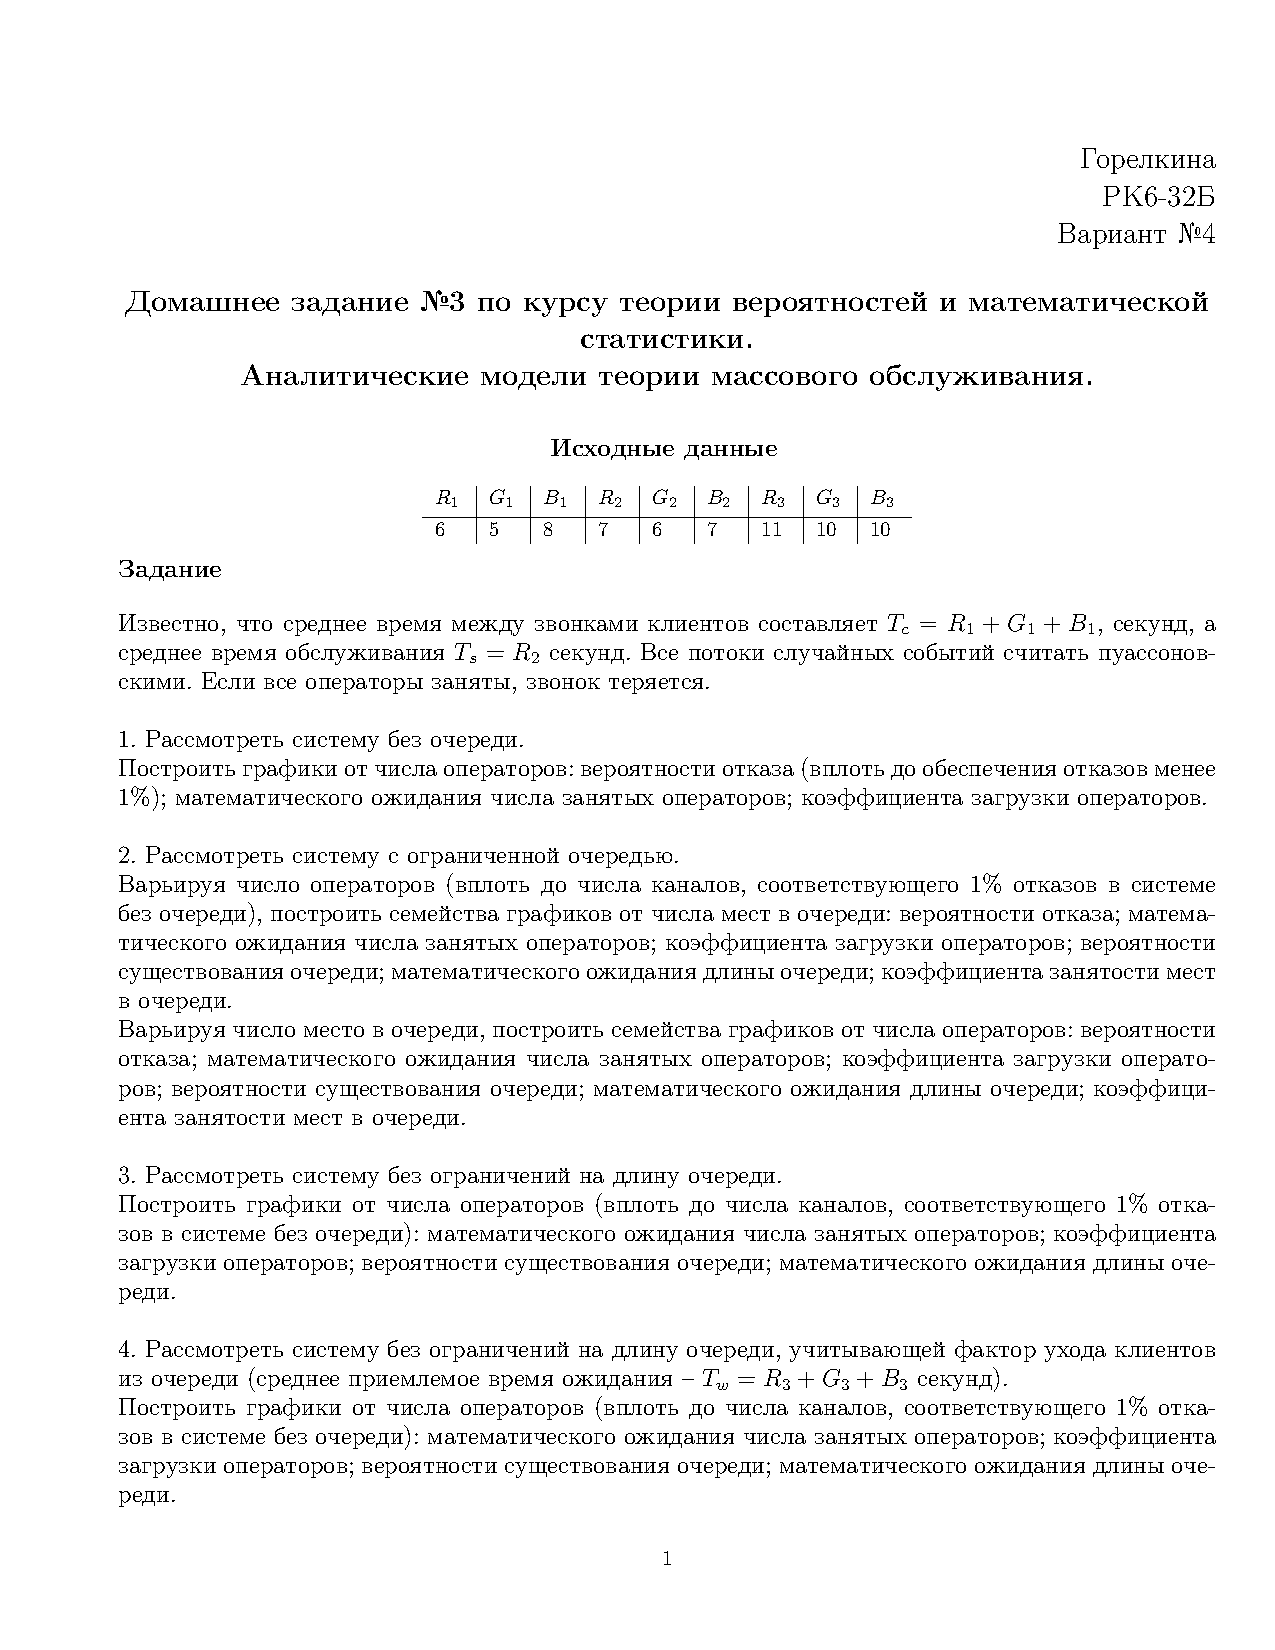
\includepdf[pages=-]{prob_3.pdf}

\end{document}